\subsection{Apresentação de Imagens}
A apresentação de imagens é definida em 2 níveis, a nível de pré-visualização, por exemplo, ver a miniatura da imagem de uma publicação no fórum e a nível de detalhe, onde é possível ver a imagem em ponto grande e realizar zoom na mesma.

Para a apresentação de miniatura da imagem foi decidido mostrar até 4 imagens, sendo que acima de 4 imagens será mostrado apenas 3 imagens significando assim que a quarta imagem indicaria quantas mais existem para mostrar. 

Para a implementação da apresentação das miniaturas de imagens, foi utilizada a biblioteca \textit{staggered\_grid\_view}, esta permite organizar imagens em grelha. Neste contexto desejava-se organizar estas imagens em diferentes aspetos, e disposições, pelo que esta biblioteca permite indicar quantas colunas e linhas existem na grelha ao criar o agrupamento de imagens. Pelo que, foi decidido que quando são duas imagens estas dividem a grelha, quando são três imagens a primeira divide metade da grelha e as outras duas dividem a outra metade, quando são 4 ou mais então as 4 dividem a grelha por igual. Quando encontram-se existentes mais do que 4 imagens, foi então decidido colocar um filtro de desfoque sobre a última imagem e colocar por cima desta quantas mais imagens existem para mostrar.

\begin{figure}[htb]%
  \centering
  \subfloat[\centering Publicação com 5 imagens]{{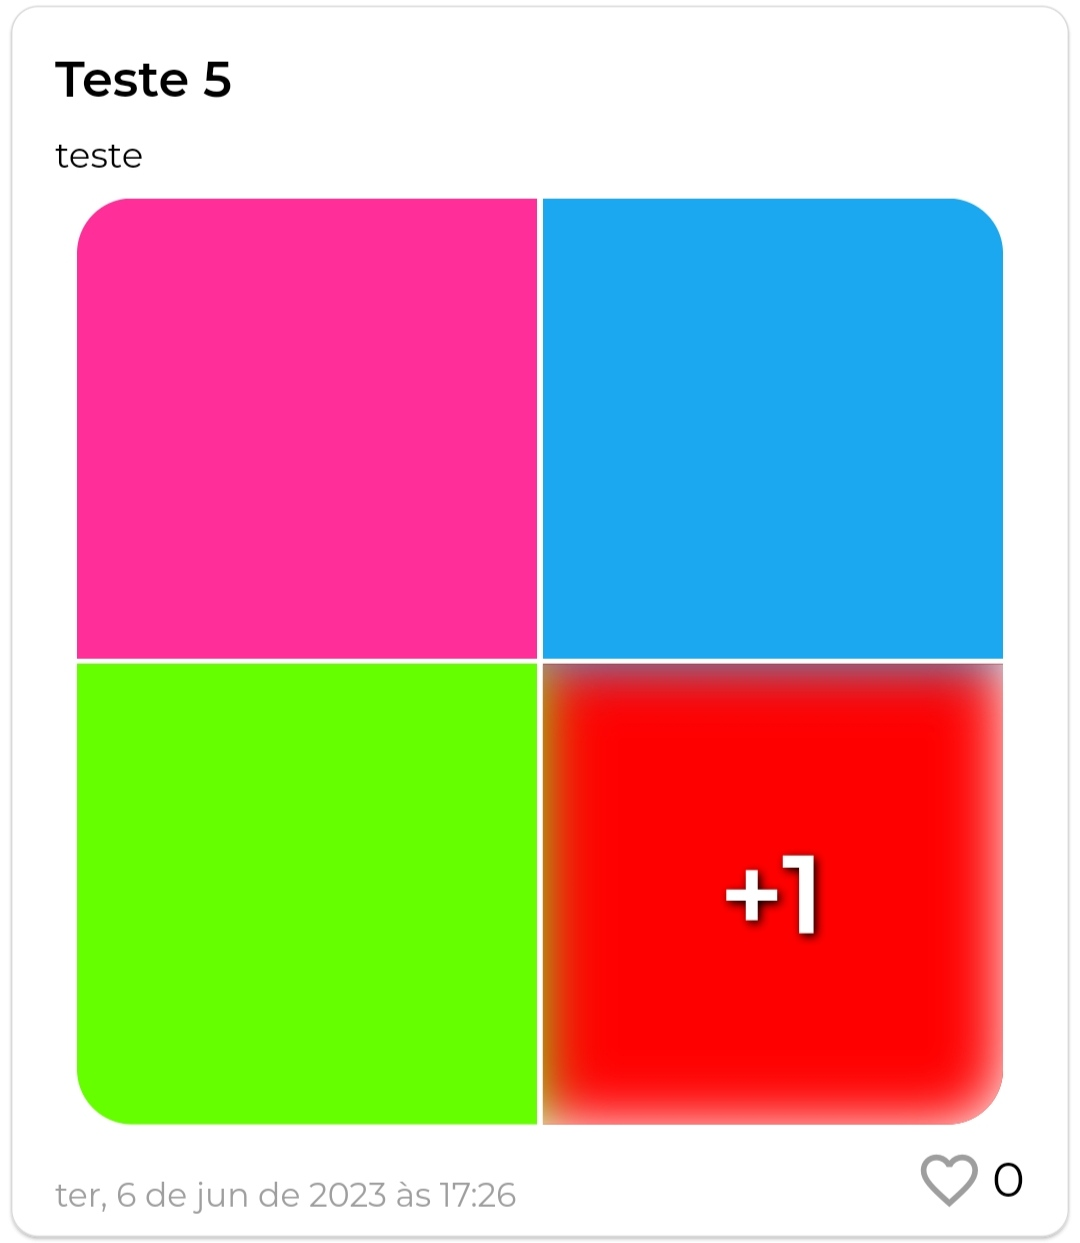
\includegraphics[width=0.25\textwidth]{images/implementacao/frontend/apresentacao_imagens/1686068843028.jpg} }}%
  \qquad
  \subfloat[\centering Publicação com 4 imagens]{{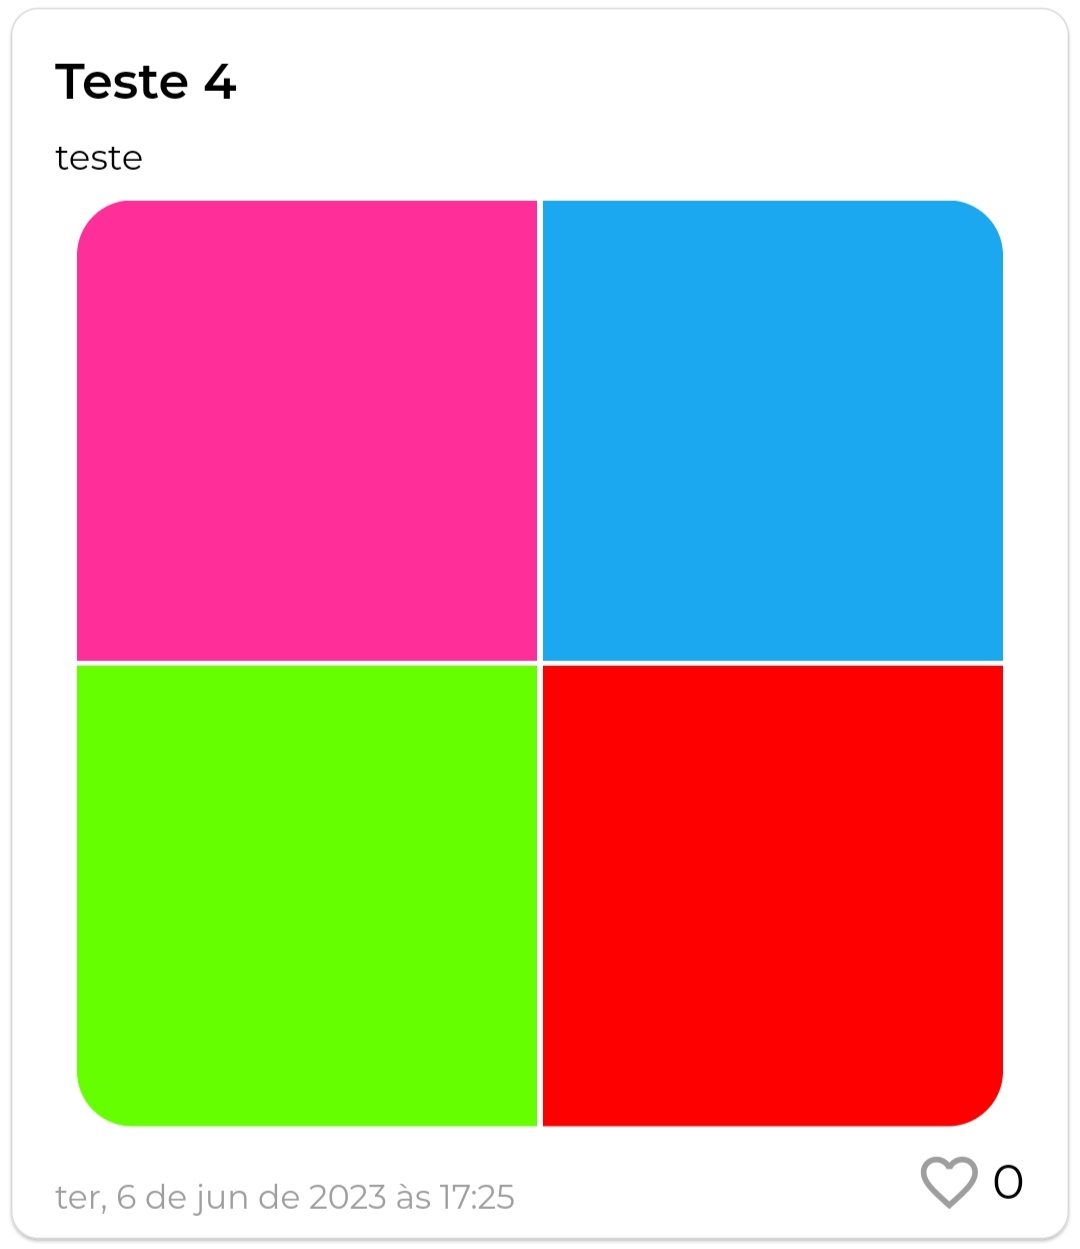
\includegraphics[width=0.25\textwidth]{images/implementacao/frontend/apresentacao_imagens/1686068843039.jpg} }}%
  \qquad
  \subfloat[\centering Publicação com 3 imagens]{{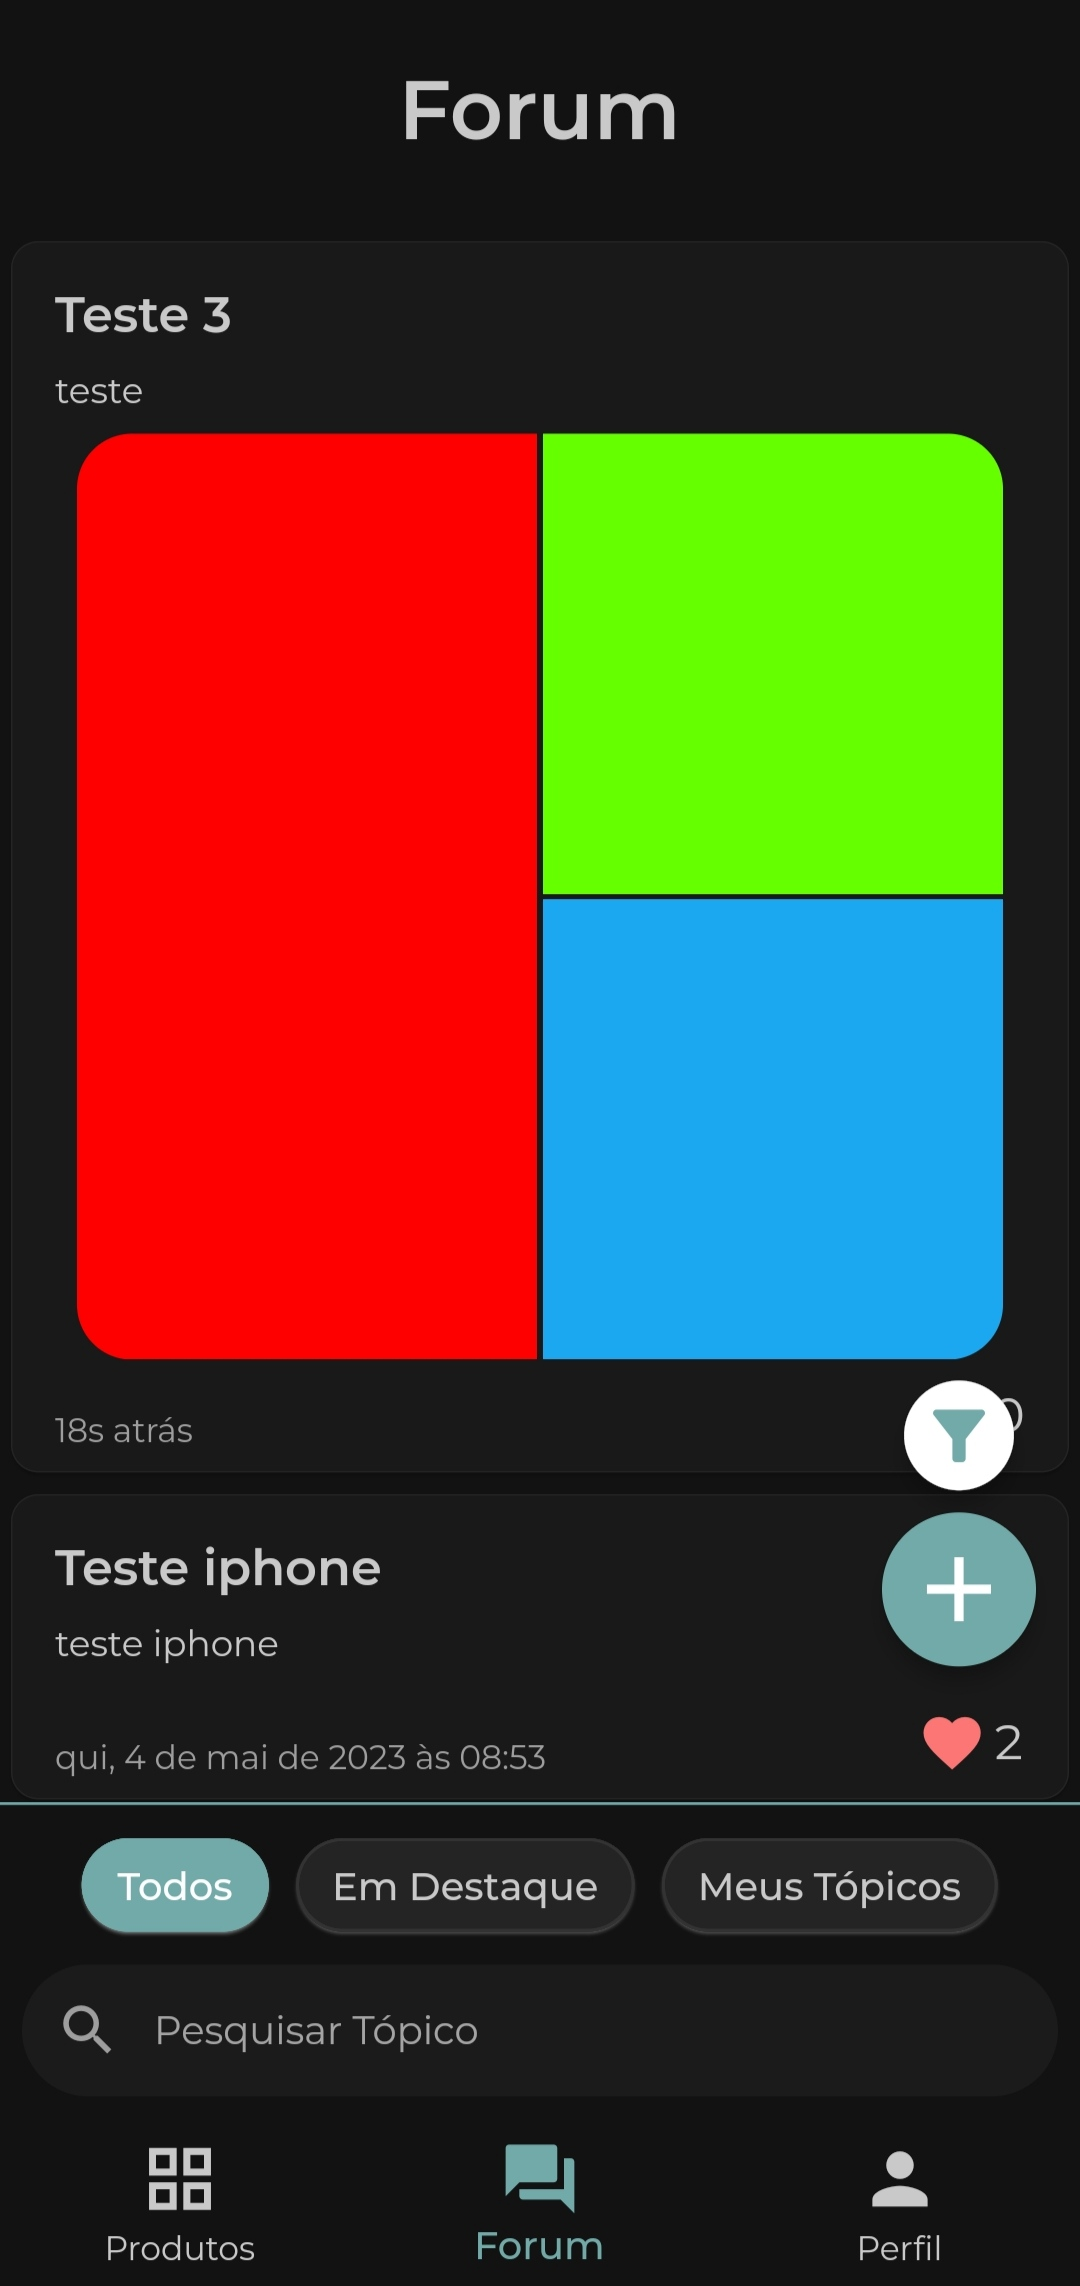
\includegraphics[width=0.25\textwidth]{images/implementacao/frontend/apresentacao_imagens/1686068843051.jpg} }}%
  \qquad
  \subfloat[\centering Publicação com 2 imagens]{{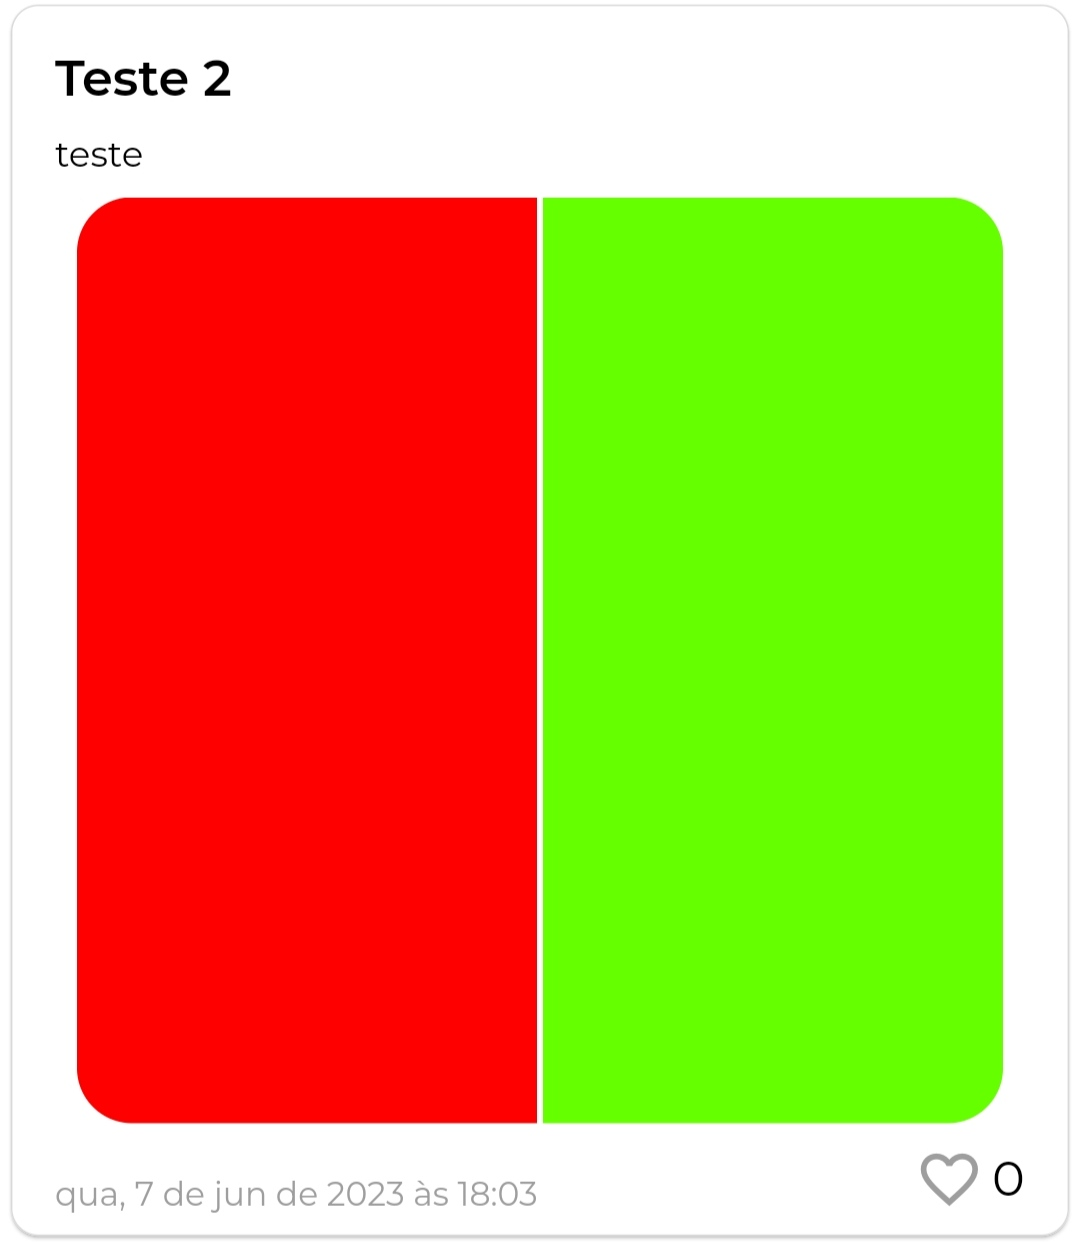
\includegraphics[width=0.25\textwidth]{images/implementacao/frontend/apresentacao_imagens/1686845317274.jpg} }}%
  \qquad
  \subfloat[\centering Publicação com 1 imageM]{{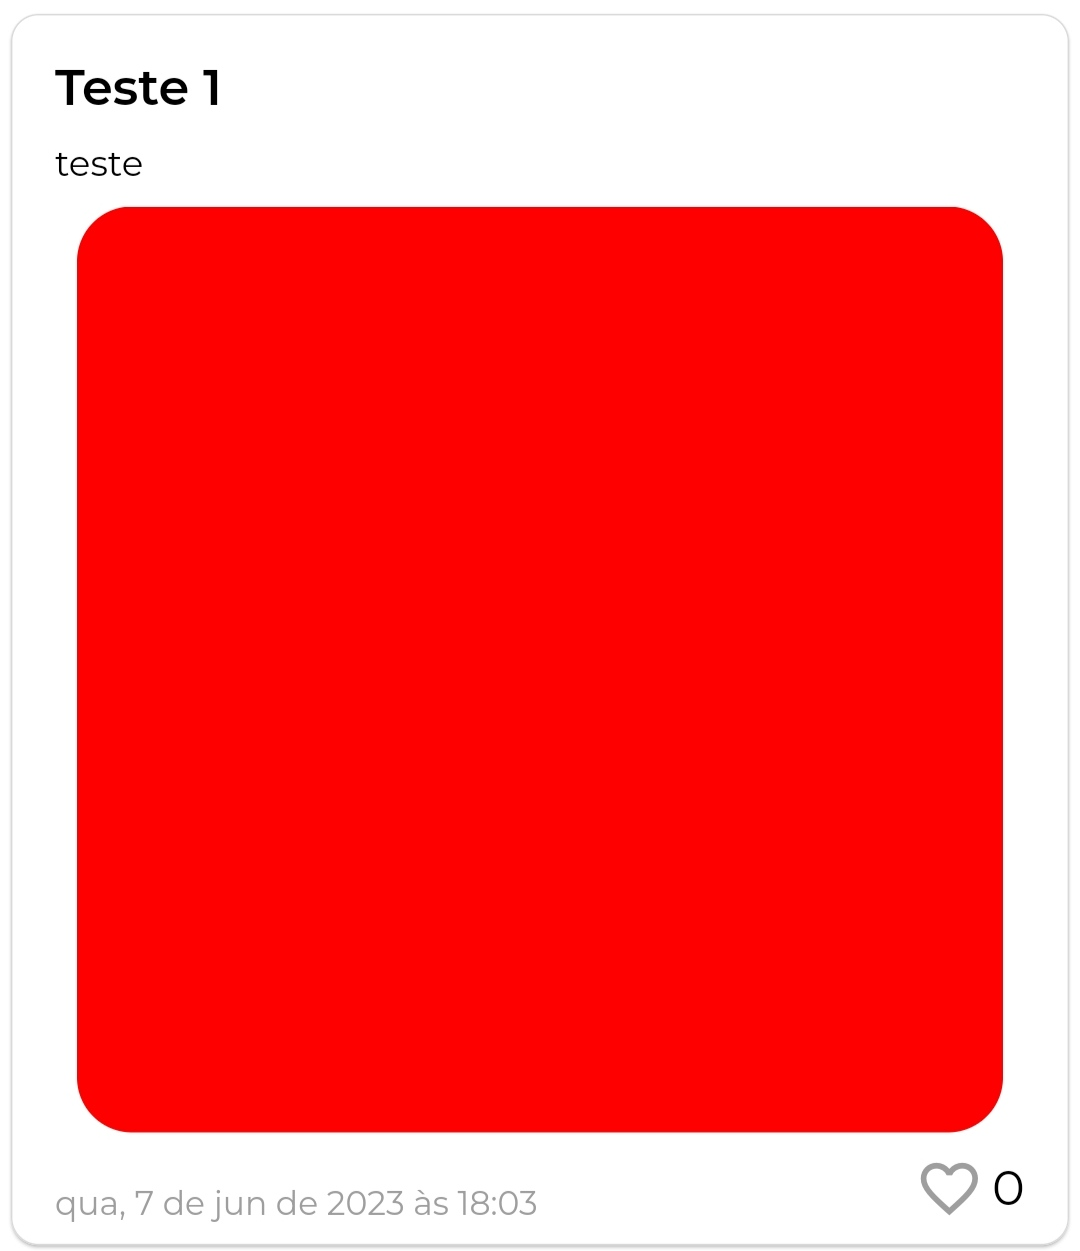
\includegraphics[width=0.25\textwidth]{images/implementacao/frontend/apresentacao_imagens/1686845317288.jpg} }}%
  \label{fig:77}%
\end{figure}

\newpage

\subsection{Apresentação de Imagens em carrosel}

A apresentação de imagens deverá permitir que o utilizador as visualize em ponto grande e realize diversas ações sobre estas. Para isso foram experimentadas diversas bibliotecas, mas nunca se conseguia o comportamento desejado, sendo assim foi decidido criar o próprio carrossel de imagens, sendo que o próprio \textit{Flutter} já disponibiliza um \textit{widget} para tal.

O ponto de maior dificuldade para este processo foi a implementação de \textit{zoom}, visto que o \textit{Flutter} não dispõe de \textit{widgets} para tal. Por isso foi necessário primeiramente detetar gestos com o detetor de gestos da ferramenta e aplicado um \textit{zoom} sobre o centro do gesto. Os gestos aceites foram o de pinça e o gesto de duplo clique.

O grande problema com esta solução é que visto que é permitido um \textit{scroll} horizontal de imagens, os gestos por vezes poderão não funcionar corretamente, principalmente o gesto de pinça que se efetuado na horizontal poderá resultar em \textit{scroll}. Para resolver tal problema foi decidido que quando dois dedos são detetados no ecrã a navegação horizontal fica bloqueada e assim que estes são levantados, a navegação horizontal é ativada novamente.

\subsection{Carregamento de Imagens}

O carregamento de imagens do dispositivo poderá ser realizado por meio de seleção da galeria. Para realizar esta seleção, em primeiro lugar, foi testada a biblioteca \textit{image\_picker}, mas esta biblioteca utiliza o seletor de ficheiro do dispositivo, o problema é que permite a seleção de qualquer tipo de ficheiros o que faz com que seja necessário um conjunto de outras verificações para garantir que apenas as imagens são selecionadas, o que levaria a uma possível perda de desempenho e de qualidade na experiência de utilização.

Sendo assim foi de seguida testada a biblioteca \textit{advanced\_image\_picker}, mas o problema desta biblioteca é que não permite selecionar vídeos. Foi de seguida decidido experimentar a biblioteca \textit{wechat\_asset\_picker}, esta cria uma página própria para seleção de imagens e vídeos diretamente da galeria. Permite também indicar o limite máximo de seleção e os tipos de ficheiros que o utilizador poderá selecionar para que apenas os tipos aceites sejam mostrados. Por fim, o único ponto desvantajoso é que não é possível traduzir o botão de confirmação de seleção de ficheiros.

Após a carregar os ficheiros para memória, estes são enviados para o \textit{firestorage} como mencionado anteriormente.